\begin{figure}[!htb]
    \begin{center}
    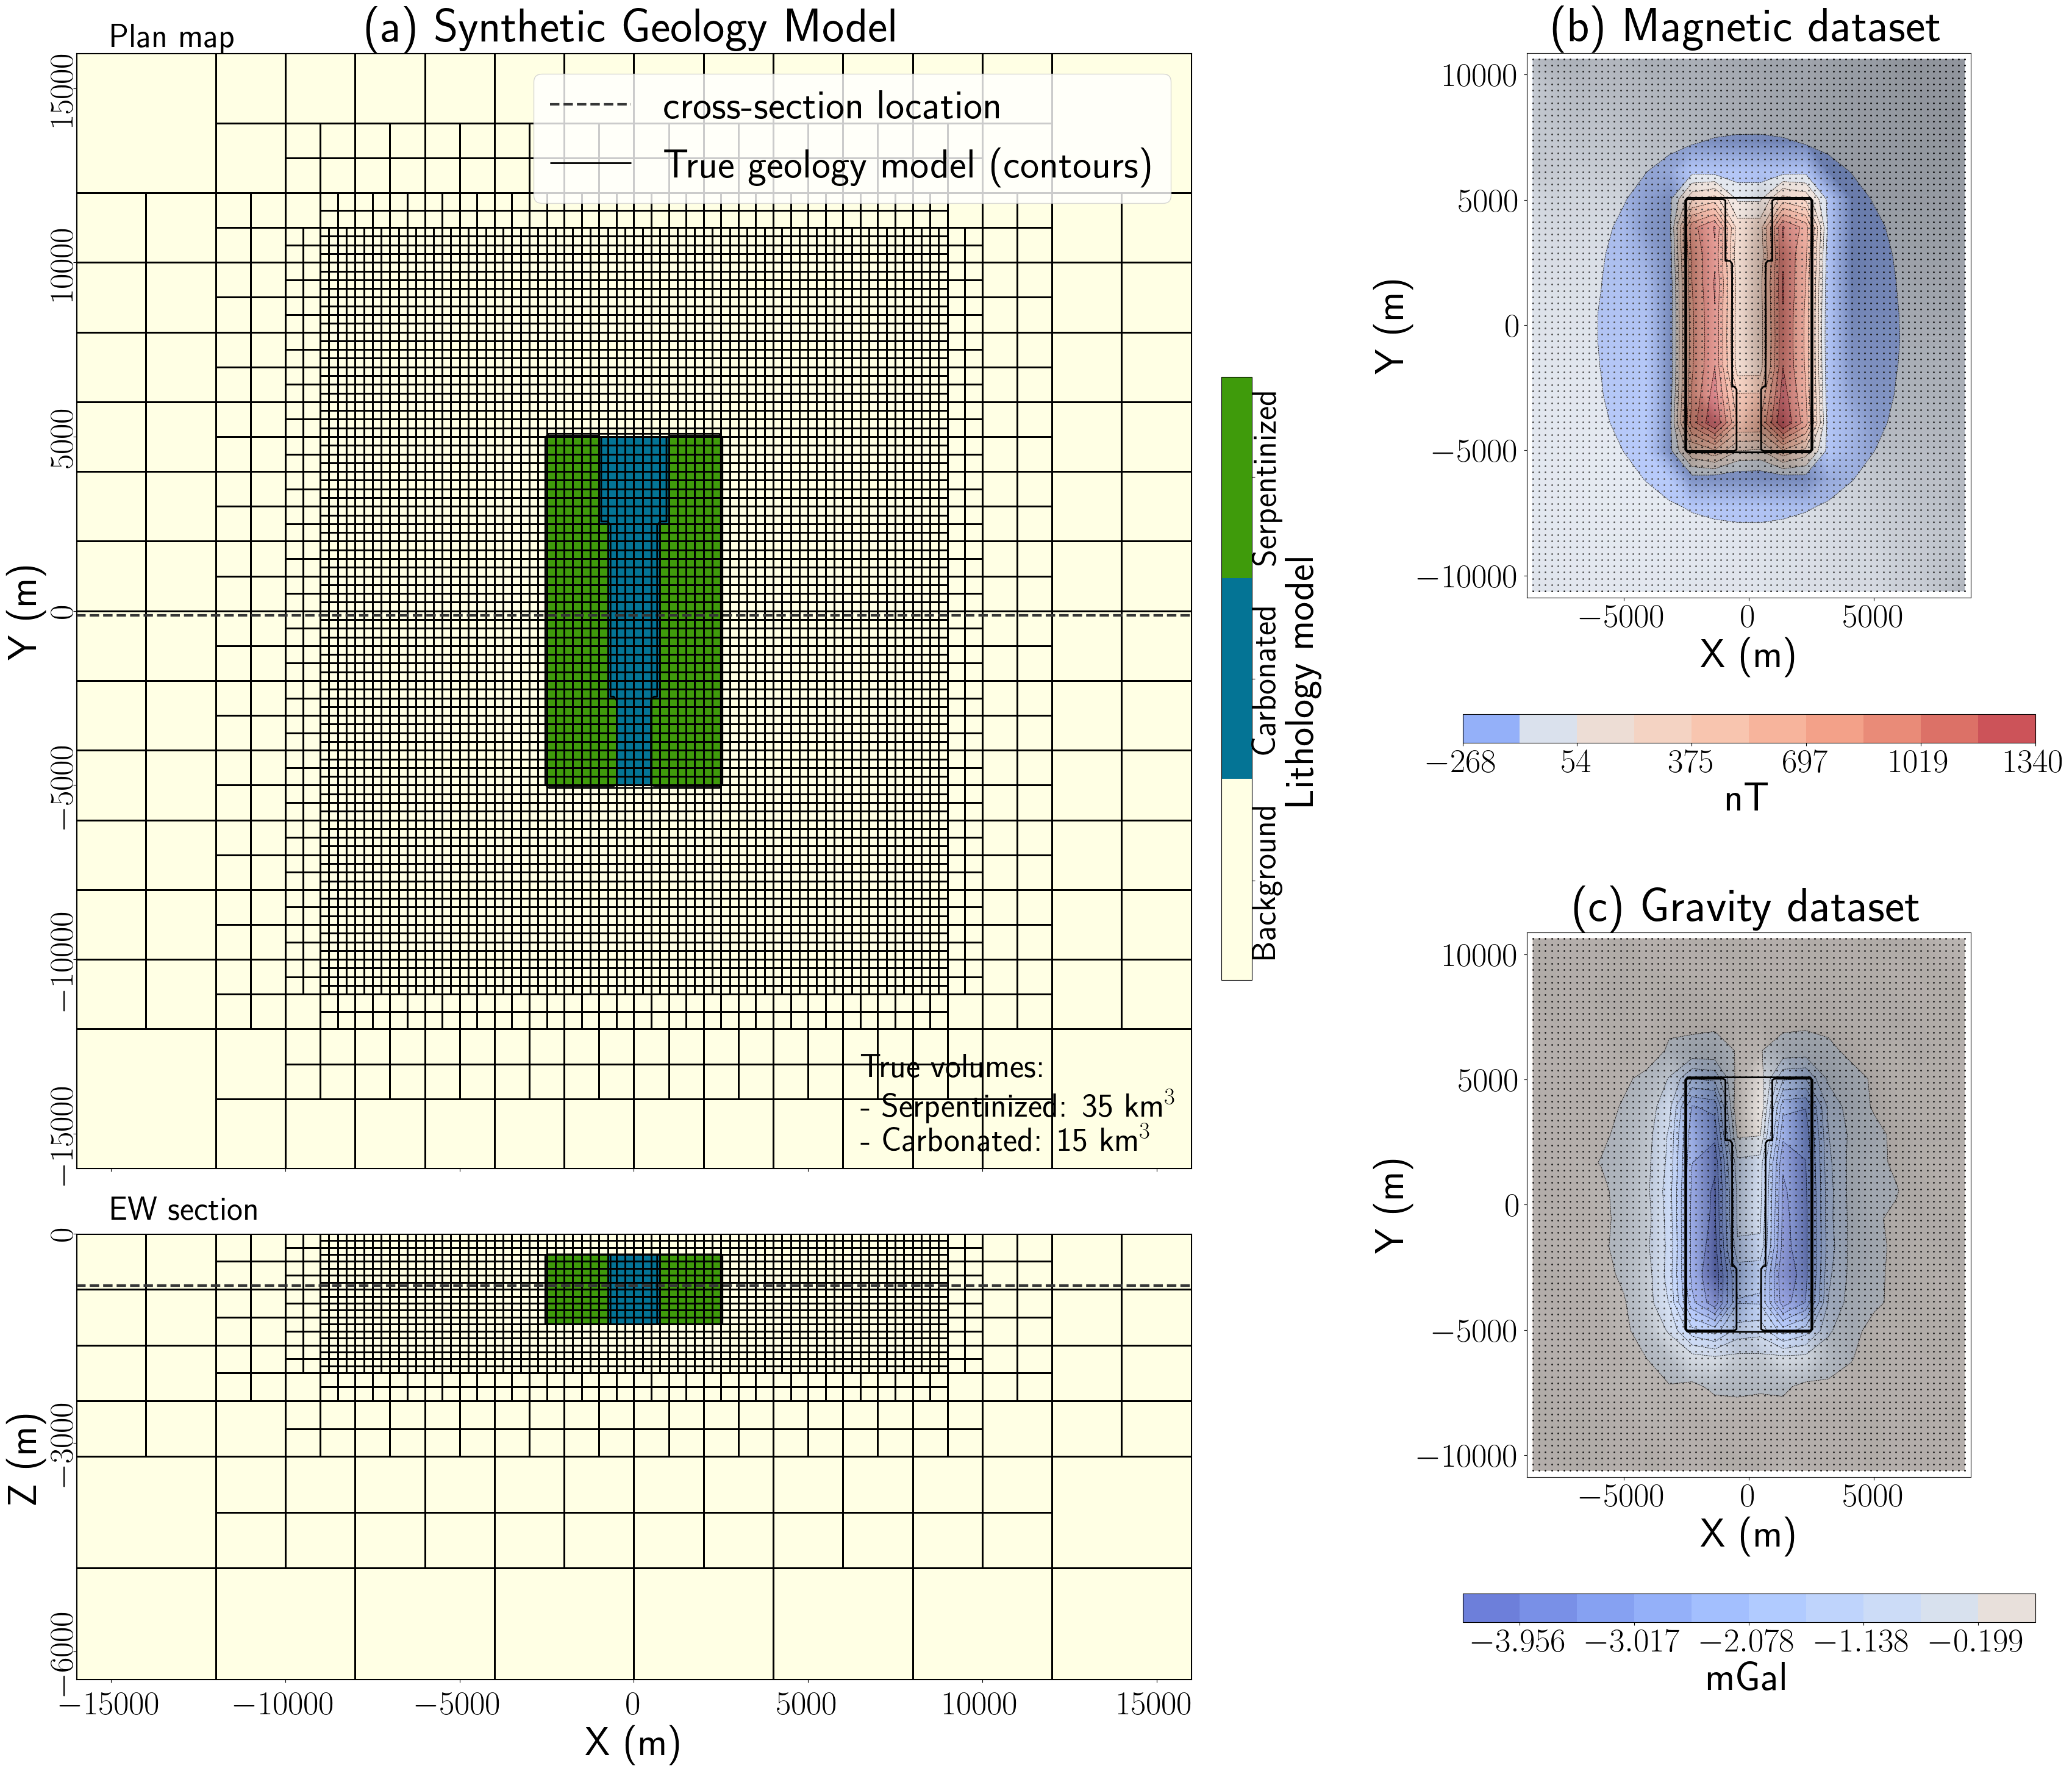
\includegraphics[width=0.6\textwidth]{figures/synthetic-three-blocks-model.png}
    \end{center}
\caption{
    (a) Representative model of a serpentinized rock unit that contains a center region that has been carbonated. The physical properties assigned to each unit are shown in table \ref{tab:physical-properties}. The total volume of serpentinized rock is 35 km$^3$ and carbonated rock is 15 km$^3$. Panels show the simulated (b) magnetic and (c) gravity data.
}
\label{fig:representative-model}
\end{figure}
